\documentclass{article}
\usepackage{Sweave}
\usepackage{amsmath}
\usepackage{amscd}
\usepackage[tableposition=top]{caption}
\usepackage{ifthen}
\usepackage[utf8]{inputenc}
\usepackage{hyperref}
\usepackage[usenames]{color}
\definecolor{midnightblue}{rgb}{0.098,0.098,0.439}
\DefineVerbatimEnvironment{Sinput}{Verbatim}{xleftmargin=2em, fontshape=sl,formatcom=\color{midnightblue}}
\DefineVerbatimEnvironment{Soutput}{Verbatim}{xleftmargin=2em}
\DefineVerbatimEnvironment{Scode}{Verbatim}{xleftmargin=2em}
\fvset{listparameters={\setlength{\topsep}{0pt}}}
\renewenvironment{Schunk}{\vspace{\topsep}}{\vspace{\topsep}}

\begin{document}
\title{Pathway fingerprint statistics}
\author{Gabriel Altschuler}
\maketitle
This document summarizes the arrays and pathways of the Pathway Fingerprint.
\section{Pathway sources}
\subsection{Canonical pathways}
Gene sets corresponding to canonical pathways were compiled from Reactome (\url{www.reactome.org}), Wikipathways (\url{www.wikipathways.org}) and KEGG (\url{www.genome.jp/kegg}). For the major signaling pathways, the transcriptionally-regulated genes (downstream targets) were obtained from Netpath (\url{www.netpath.org}).
\subsection{Functional Interaction Modules}
A Functional Interaction (FI) network was constructed by extending curated pathways with non-curated sources of information, including protein-protein interactions, gene co-expression, protein domain interaction, Gene Ontology (GO) annotations and text-mined protein interactions, all of which together cover close to half of the human proteome (\emph{Wu et al., 2010}). The network was decomposed by applying a Markov Cluster Algorithm (MCL) (\emph{Enright et al 2002}), yielding 144 closely related functional interaction clusters ranging from 10 to 743 nodes. Each cluster was named according to the member gene with the highest interaction degree. For more information contact Irina Kalatskaya and Lincoln Stein.
\subsection{Cross-species conversion}
A total of 633 \emph{Homo sapiens} gene sets were assembled. Corresponding gene sets for \emph{M. musculus}, \emph{R. norvegicus}, \emph{D. rerio}, \emph{D. melanogaster} and \emph{C.elegans} were inferred by homology (Homologene, \url{www.ncbi.nlm.nih.gov/homologene}).
\begin{Schunk}
\begin{Sinput}
> library(pathprint)
\end{Sinput}
\end{Schunk}
\section{Pathway sets}
The human pathway set contains 633 pathways.
\begin{Schunk}
\begin{Sinput}
> pathway.info<-as.data.frame(
   matrix(nrow = 6, ncol = 5,
   dimnames = list(c(names(genesets)[1:6]),
                   c("nGenes", "MeanLength",
                     "MedianLength", "MinLength", "MaxLength"
                     ))))
> for (i in rownames(pathway.info)){
   pathways<-get(genesets[i])
   pathway.info[i, "nGenes"] <- length(unique(unlist(pathways)))
   pathway.info[i, "MeanLength"] <- round(mean(sapply(pathways, length)),2)
   pathway.info[i, "MedianLength"] <- median(sapply(pathways, length))
   pathway.info[i, "MinLength"] <- min(sapply(pathways, length))
   pathway.info[i, "MaxLength"] <- max(sapply(pathways, length))
   }
\end{Sinput}
\end{Schunk}
% latex table generated in R 2.11.1 by xtable 1.5-6 package
% Thu May 17 16:37:11 2012
\begin{table}[tbp]
\begin{center}
\caption{Pathway statistics by species}
\label{Tab_speciesTab}
\begin{tabular}{rrrrrr}
  \hline
 & nGenes & MeanLength & MedianLength & MinLength & MaxLength \\ 
  \hline
Homo sapiens & 10903 & 73.53 &  41 &   6 & 1138 \\ 
  Mus musculus & 8951 & 65.80 &  37 &   5 & 1074 \\ 
  Rattus norvegicus & 8312 & 62.03 &  35 &   3 & 1002 \\ 
  Drosophila melanogaster & 2927 & 23.84 &  12 &   0 & 560 \\ 
  Danio rerio & 6749 & 51.77 &  30 &   1 & 901 \\ 
  Caenorhabditis elegans & 2284 & 18.88 &  10 &   0 & 470 \\ 
   \hline
\end{tabular}
\end{center}
\end{table}\begin{figure}
\begin{center}
\begin{Schunk}
\begin{Sinput}
> par(mfcol = c(2,3))
> for (i in rownames(pathway.info)){
   pathways<-get(genesets[i])
   #hist(log(sapply(pathways, length),10), breaks = seq(0,3.2,0.2),
   #     xlim = c(0,log(1200, 10)))
   hist<-hist(sapply(pathways, length), breaks = c(0, 10^seq(-0.1,log(3000,10), 0.1)),
        plot = FALSE)
   plot(hist$counts ~ hist$mids, log = "x", type = "h", xaxt = "n",
        xlab = "Pathway size", ylab = "Frequency",
        main = i)
   axis(1, hist$mids, round(signif(hist$mids, 2)))
   }
\end{Sinput}
\end{Schunk}
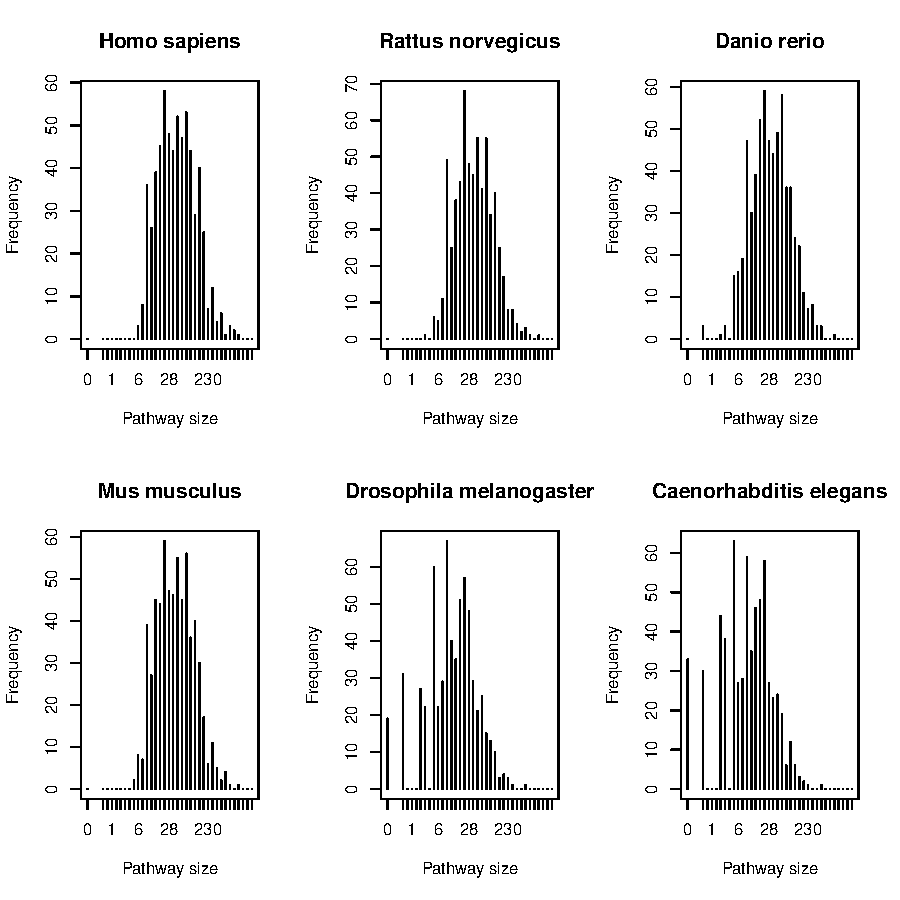
\includegraphics{pathwayStats-pathwaySizePlot}
\end{center}
\caption{Histograms of pathway sizes}
\label{fig:pathwaySizePlot}
\end{figure}

\begin{Schunk}
\begin{Sinput}
> types<-c("Reactome",
          "Wikipathways",
          "Netpath",
          "KEGG",
          "Static Module",
          "All")
> pathway.type<-as.data.frame(
   matrix(nrow = 6, ncol = 5,
   dimnames = list(types,
                   c("nGenes", "MeanLength",
                     "MedianLength", "MinLength", "MaxLength"
                     ))))
> for (i in types[1:5]){
   pathways<-pathprint.Hs.gs[grep(i, names(pathprint.Hs.gs))]
   pathway.type[i, "nGenes"] <- length(unique(unlist(pathways)))
   pathway.type[i, "MeanLength"] <- round(mean(sapply(pathways, length)),2)
   pathway.type[i, "MedianLength"] <- median(sapply(pathways, length))
   pathway.type[i, "MinLength"] <- min(sapply(pathways, length))
   pathway.type[i, "MaxLength"] <- max(sapply(pathways, length))
   }
> for (i in types[6]){
   pathways<-pathprint.Hs.gs
   pathway.type[i, "nGenes"] <- length(unique(unlist(pathways)))
   pathway.type[i, "MeanLength"] <- round(mean(sapply(pathways, length)),2)
   pathway.type[i, "MedianLength"] <- median(sapply(pathways, length))
   pathway.type[i, "MinLength"] <- min(sapply(pathways, length))
   pathway.type[i, "MaxLength"] <- max(sapply(pathways, length))
   }
> types <- types[1:5]
\end{Sinput}
\end{Schunk}
% latex table generated in R 2.11.1 by xtable 1.5-6 package
% Thu May 17 16:37:12 2012
\begin{table}[tbp]
\begin{center}
\caption{Pathway statistics by type (human genesets)}
\label{Tab_typeTab}
\begin{tabular}{rrrrrr}
  \hline
 & nGenes & MeanLength & MedianLength & MinLength & MaxLength \\ 
  \hline
Reactome & 4874 & 153.60 & 108.00 &  11 & 932 \\ 
  Wikipathways & 3918 & 50.14 & 33.00 &   6 & 260 \\ 
  Netpath & 3811 & 170.08 & 83.00 &   8 & 816 \\ 
  KEGG & 5990 & 75.51 & 55.00 &   6 & 1138 \\ 
  Static Module & 6458 & 44.90 & 21.00 &   9 & 733 \\ 
  All & 10903 & 73.53 & 41.00 &   6 & 1138 \\ 
   \hline
\end{tabular}
\end{center}
\end{table}\begin{Schunk}
\begin{Sinput}
> overlap<-matrix(nrow = 5, ncol = 5, dimnames = list(types, types))
> types.genes<-sapply(types, function(x){
   unique(unlist(pathprint.Hs.gs[grep(x, names(pathprint.Hs.gs))]))
   }
   )
> for (i in types){
  overlap[i,]<-sapply(types.genes, function(x){length(intersect(x, types.genes[[i]]))})
  }
> overlap.lower<-overlap
> overlap.lower[upper.tri(overlap.lower)]<-""
\end{Sinput}
\end{Schunk}
% latex table generated in R 2.11.1 by xtable 1.5-6 package
% Thu May 17 16:37:12 2012
\begin{table}[tbp]
\begin{center}
\caption{Overlap in gene membership between pathway types (human genesets)}
\label{Tab_overlapTab}
\begin{tabular}{rlllll}
  \hline
 & Reactome & Wikipathways & Netpath & KEGG & Static Module \\ 
  \hline
Reactome & 4874 &  &  &  &  \\ 
  Wikipathways & 2402 & 3918 &  &  &  \\ 
  Netpath & 1652 & 1646 & 3811 &  &  \\ 
  KEGG & 3494 & 2814 & 2011 & 5990 &  \\ 
  Static Module & 3190 & 2526 & 2052 & 3514 & 6458 \\ 
   \hline
\end{tabular}
\end{center}
\end{table}
\end{document}
